% \begin{frame}[fragile]{Интерфейс рабочей среды системы}
% \begin{columns}

% \begin{column}{0.3\textwidth}
% Интерфейс системы включает в себя 3D визуализацию, несколько информационных полей о начертанном графе и блок управления визуализацией и функционалом интерактивного анализа.

% % Внешний вид системы значительно изменился. Появился список с информацией о графе и возникших ошибках при его построении. В пользовательском меню появились функции управления уровнем ярусно-параллельной формы. Изменились цвета и геометрические формы объектов графа. Появился изгиб дуг в необходимых случаях.
% \end{column}

% \begin{column}{0.7\textwidth}
% \includegraphics
% % [width=\textwidth]{images/example1}\\
% [width=\textwidth]{images/screenshot_5}\\
% \end{column}

% \end{columns}
% \end{frame}



\begin{frame}[fragile]{Интерфейс рабочей среды}
\vspace{2mm}

Интерфейс включает в себя интерактивную визуализацию информационного графа, несколько информационных полей и блок управления и анализа.

\vspace{3mm}
\centering
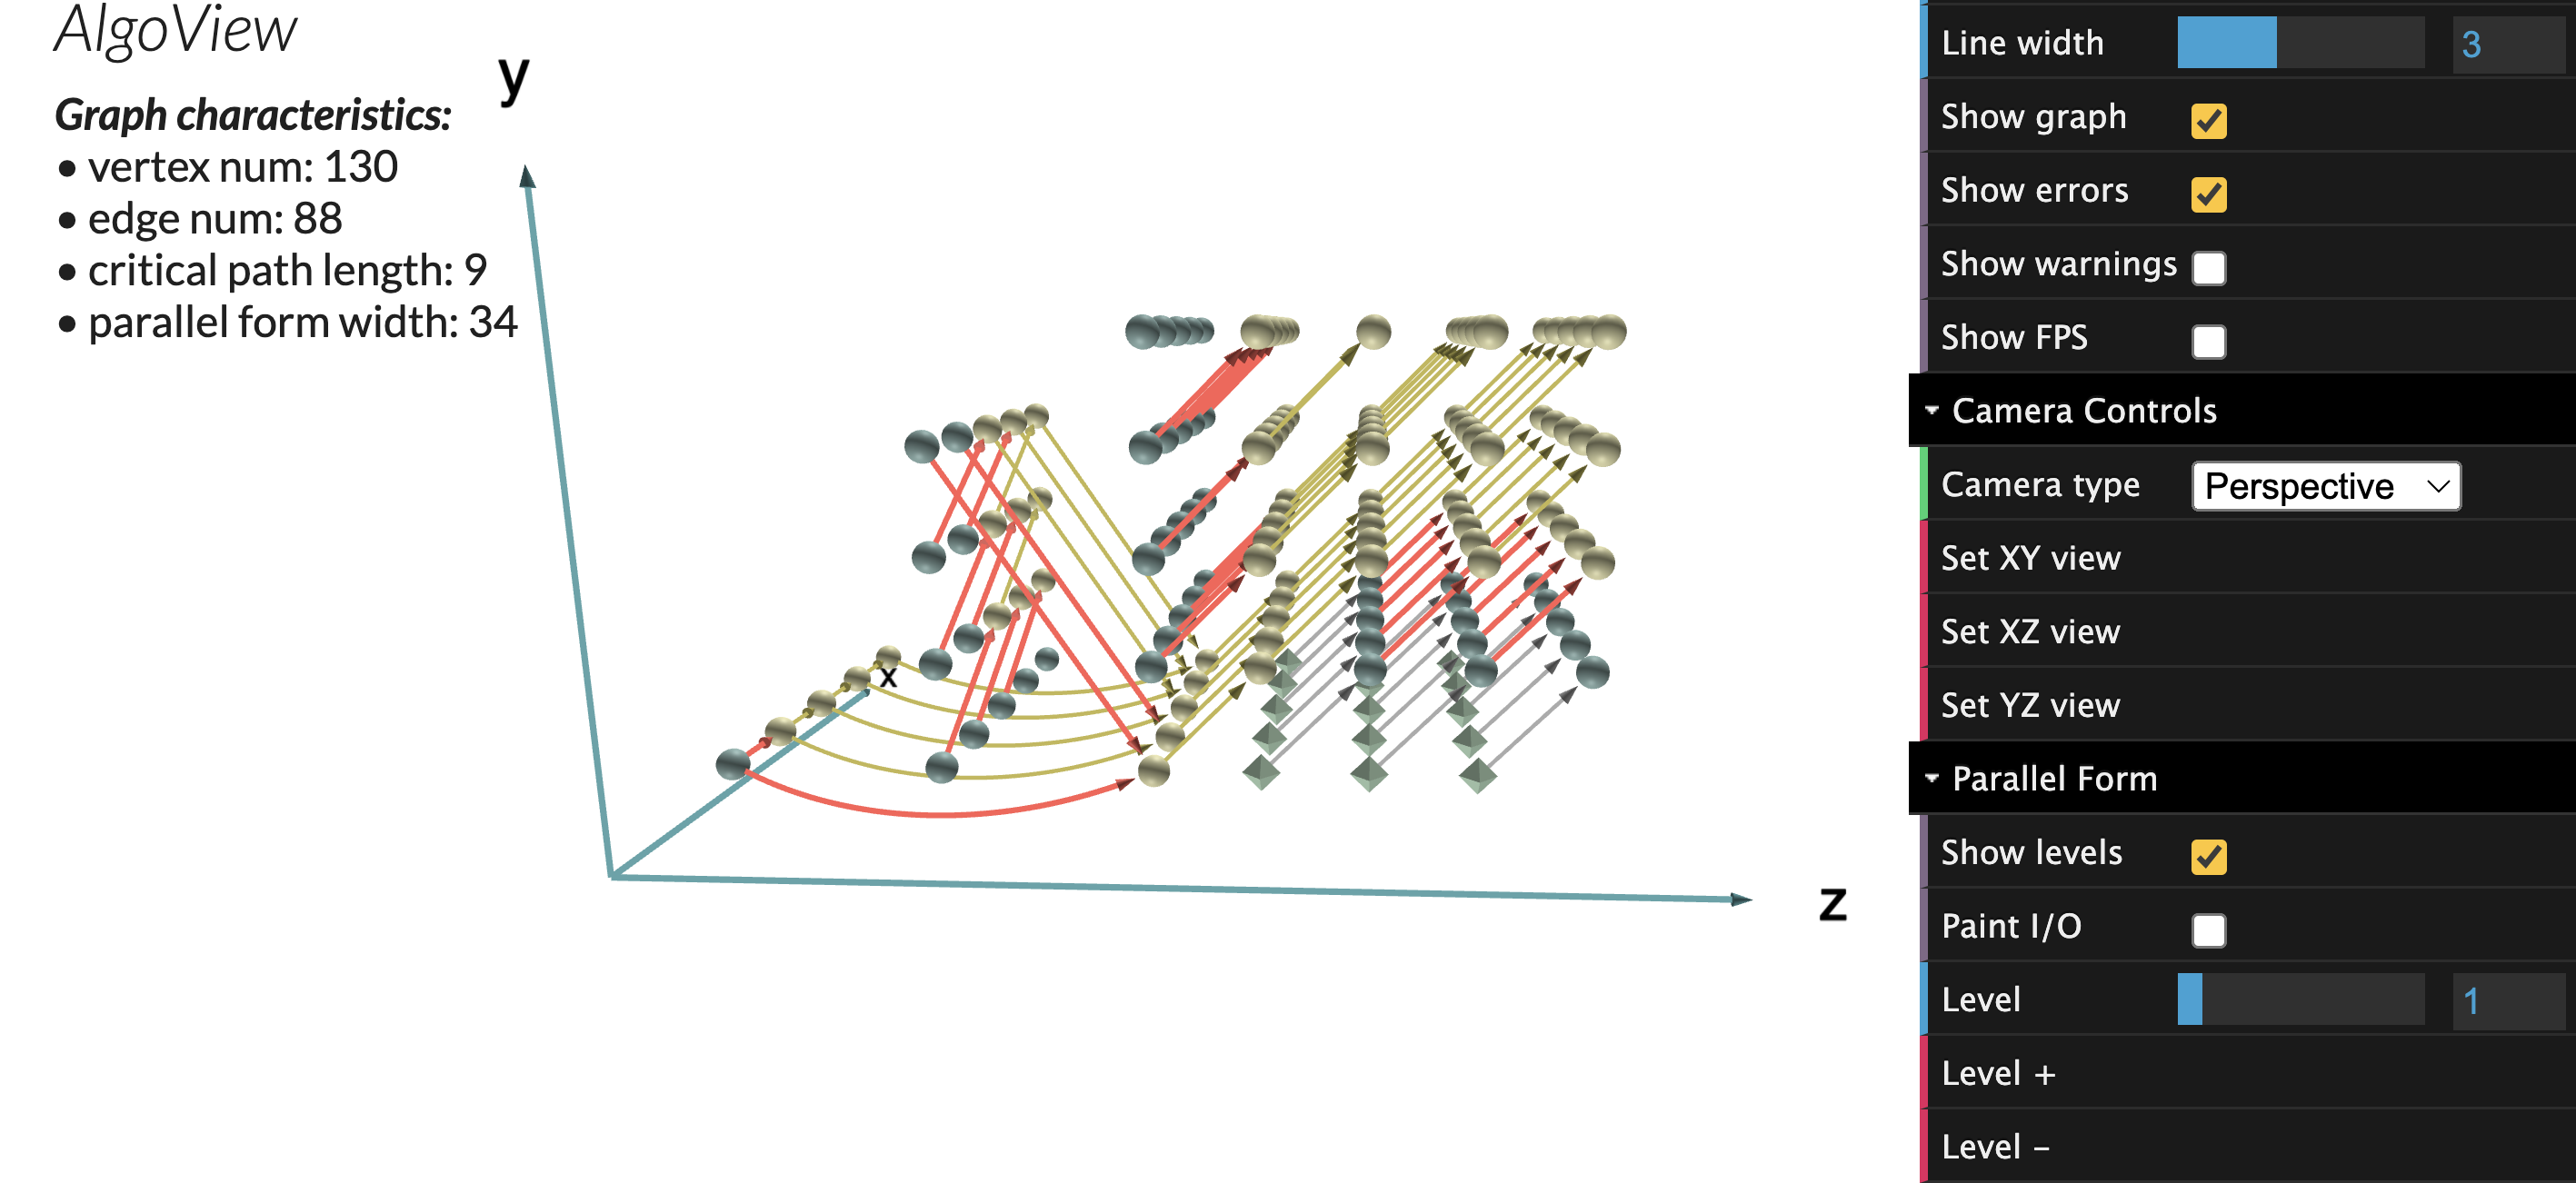
\includegraphics
[width=0.85\textwidth]{images/screenshot_6}\\

\end{frame}
